L'archiettura della piattaforma è stata ideata come segue:

\begin{center}
    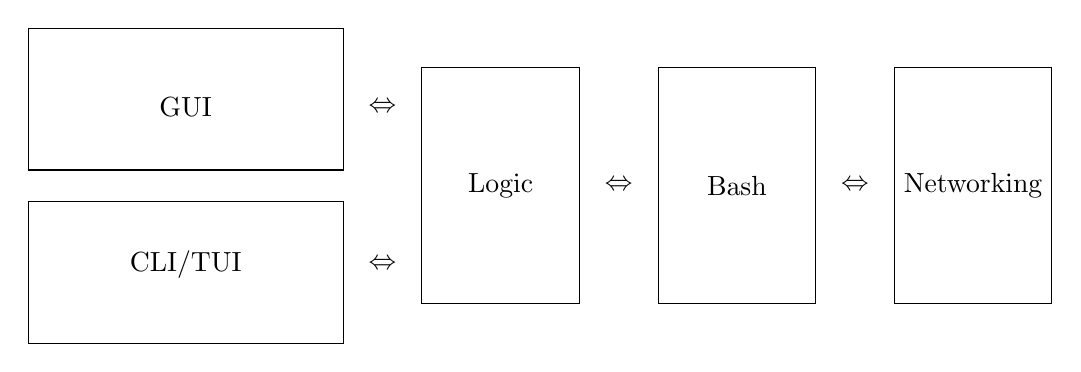
\begin{tikzpicture}
        \draw (0,0) rectangle (4,1.8);
        \draw (0,2.2) rectangle (4,4);
        \draw (5,0.5) rectangle (7,3.5);
        \draw (8,0.5) rectangle (10,3.5);
        \draw (11,0.5) rectangle (13,3.5);
        \node[] at (12,2) {Networking};
        \node[] at (9,2) {Bash};
        \node[] at (6,2) {Logic};
        \node[] at (2,3) {GUI};
        \node[] at (2,1) {CLI/TUI};
        \node[] at (10.5,2) {$\Leftrightarrow$};
        \node[] at (7.5,2) {$\Leftrightarrow$};
        \node[] at (4.5,3) {$\Leftrightarrow$};
        \node[] at (4.5,1) {$\Leftrightarrow$};
    \end{tikzpicture}
\end{center}

Le componenti che dovremmo realizzare sarebbero pertanto:
\begin{itemize}
    \item \textbf{Networking}: Utilizzo di container e apparati virtualizzati. Si tratta del modo in cui vengono realizzati, come in IMUNES, i componenti veri e propri. Essi sono poi connessi tra di loro mediante gli appositi comandi e possono simulare una rete.
    \item \textbf{Logic}: la logica del programma deve effettuare la comunicazione dei comandi dell'utente alla parte sottostante
    \item \textbf{GUI}: si tratta dell'interfaccia su cui l'utente può disegnare la topologia logica della rete, posizionando quindi nodi e link tra nodi, trascinandoli, modificandoli e interagendoci in genere
    \item \textbf{CLI/TUI}: da qui si possono lanciare i comandi di configurazione dei vari componenti. Essa aprirà un editor di testo sui file di configurazione, permettendo quindi di modificarli, salvarli e caricare le modifiche anche nella visualizzazione GUI.
\end{itemize}
Gli obiettivi che desideriamo perseguire attraverso questo progetto:\begin{itemize}
    \item \textbf{Ridurre le dipendenze} al minimo necessario, in modo da rendere il programma il più portabile possibile
    \item Fornire la \textbf{capacità di salvare} non solo la topologia fisica ma anche tutte le configurazioni, senza bisogno di script ulteriori
    \item \textbf{Uscire in modo pulito}, evitando che Docker rimanga in uno stato intermedio (ossia con i vecchi container ancora presenti) in caso di chiusura della applicazione senza arresto della simulazione
\end{itemize}



\newpage
